\section{Caratteri generali del rinascimento (XIII - XVI secolo).}\label{CaratteriGeneraliDelRinascimento}
\par La matematica del rinasciamento \`e caratterizzata dall'intreccio di tre fili, intreccio che esamineremo nelle pagine seguenti:
\begin{itemize}
	\item il primo filo \`e quello dell'aritmetica mercantile, che nasce dalla matematica di Leonardo Fibonacci e in particolare del suo \textit{Liber Abaci}, e sfocia in numerosi ambiti teorici e applicativi attraverso le scuole d'abaco (sottosezione \ref{LeonardoFibonacciELeScuoleDAbaco}), come gli studi prospettici di Piero della Francesca (circa 1416 - 1492) e la teoria delle equazioni, che preparer\`a il campo all'algebra simbolica di Fran\c{c}ois Vi\`ete (sottosezione \ref{FrancoisVieteELInvenzioneDellAlgebraSimbolica});
	\item il secondo filo \`e quello dell'umanesimo e della ricerca dei classici (sottosezione \ref{LUmanesimoEIlRecuperoDellaMatematicaGreca}), favorito dall'invenzione della stampa (sottosezione \ref{LInvenzioneDellaStampaELaDiffusioneDellaCulturaScientifica});
	\item l'ultimo filo \`e quello della tradizione dei testi filosofici antichi, in particolare della filosofia naturale (sottosezione \ref{LaTraditioDellOperaDiArchimedeDiApollonioEDiPappo}), che genera studi di fisica che favoriranno l'avvento della rivoluzione scientifica galileiana (sottosezione \ref{IlProblemaDeiCentriDiGravitaELOperaDiLucaValerio}).
\end{itemize}
\subsection{La cultura dell'abaco e dell'umanesimo.}\label{Storia_della_matematiLaCulturaDellAbacoEDellUmanesimo}
\subsubsection{Leonardo Fibonacci e le scuole d'abaco.}\label{LeonardoFibonacciELeScuoleDAbaco}
\paragraph{Biografia di Leonardo Pisano, detto Fibonacci.} Poco \`e noto della vita di Leonardo Pisano. Egli nasce a Pisa verosimilmente tra il 1170 e il 1180 e in giovane et\`a segue suo padre, il mercante Guglielmo dei Bonacci, nella citt\`a di Bugia (odierna Algeria). Guglielmo \`e stato incaricato dal comune di Pisa di svolgere a Bugia le funzioni di \textit{publicus scriba pro pianis mercatoribus}, in un'epoca in cui Pisa, una delle famose repubbliche marinare, vanta un'importantissima presenza in tutto il Mediterraneo.
\par Guglielmo manda suo figlio Leonardo a studiare presso maestri arabi di matematica e il Fibonacci acquista le nuove conoscenze con grandissimo interesse, tanto da decidere di percorrere tutto il Mediterraneo alla ricerca di conoscenze aggiuntive: il risultato \`e l'opera pi\`u famosa di Fibonacci, l'enciclopedico \textit{Liber abaci} (1202), che descriveremo in dettaglio in seguito.
\par Il \textit{Liber abaci}, dopo poche iniziali difficolt\`a, si impone rapidamente come modello di manuale di aritmetica mercantile, tanto da portare alla fondazione di numerose scuole d'abaco, col preciso intento di insegnarne i contenuti. Leonardo stesso diventa maestro d'abaco, come dimostra chiaramente un documento datato del 1241 che lo assume presso il comune di Pisa con questa funzione.
\par Fibonacci scrive altre opere, tra cui la pi\`u importante \`e la \textit{Practica geometriae} (1220), un trattato di geometria da cui i maestri d'abaco traggono talvolta materiale per le loro lezioni. Intrattiene inoltre rapporti con Federico II di Svevia e la sua corte, tanto che molte delle sue opere sono dedicate a suoi membri. La data di morte \`e ignota.
\paragraph{Il \textit{Liber abaci}.} Il \textit{Liber abaci} \`e senza dubbio il pi\`u importante dei lavori di Fibonacci, prima di tutto per influenza. Il suo contenuto consiste in un'esposizione di tutta l'aritmetica araba sino circa ad Ab\=u K\=amil (circa 850 - circa 930), con l'importante influenza dei lavori di al-Khw\=arizm\={\i} (circa 780 - circa 850). Questa \`e la struttura del \textit{Liber abaci}:
\begin{itemize}
	\item capitoli 1-7: aritmetica -- cifre araboindiane, notazione posizionale, operazioni tra numeri interi e frazioni;
	\item capitoli 8-11: aritmetica mercantile -- cambi, pesi e misure, compravendita, baratti, distribuzione di profitti in societ\`a, fusione di monete;
	\item capitolo 12: curiosit\`a matematiche -- per esempio comprende la successione di Fibonacci derivata dal famoso problema dei conigli e il metodo della falsa posizione per la risoluzione di problemi che conducono a equazioni lineari del tipo $ax = b$;
	\item capitoli 13: il metodo della doppia falsa posizione per la risoluzione di problemi che conducono ad equazioni lineari del tipo $ax + b = c$;
	\item capitolo 14: estrazione di radici quadrate e cubiche;
	\item capitolo 15: proporzioni geometriche e algebra.
\end{itemize}
\par Lo stile dell'opera \`e retorico: il formalismo matematico \`e ancora molto rudimentale e si limita a fornire soluzioni sotto forma di ricette con un linguaggio pi\`u o meno uniforme.
\par Forniamo una breve descrizione della dimostrazione delle formule di risoluzione delle equazioni di secondo grado secondo gli arabi e dunque secondo Fibonacci. Innanzitutto, bisogna ricordare che la matematica araba non considera mai quantit\`a negative (neanche come soluzioni; anzi, spesso viene trascurata anche la soluzione nulla), pertanto le equazioni di secondo grado vengono per prima cosa classificate in forme normali, che riportiamo in notazioni moderne:
\begin{itemize}
	\item $ax^2 = bx$;
	\item $ax^2 = c$;
	\item $bx = c$;
	\item $ax^2 + c = bx$;
	\item $ax^2 + bx = c$;
	\item $ax^2 = bx + c$.
\end{itemize}
\par Le prime tre equazioni si risolvono facilmente con estrazioni di radici e metodo della falsa posizione. Le altre tre vengono ulteriormente normalizzate dividendo per $a$ (i \textit{censi}, cio\`e la quantit\`a di \textit{censi} cio\`e di quadrati dell'incognit\`a\footnote{L'incognita alla prima potenza si chiama invece \textit{radice} e la costante \textit{numero}; analogamente per \textit{radici} si intende la quantit\`a di radici dell'equazione, cio\`e $b$.}):
\begin{itemize}
	\item $x^2 + c = bx$;
	\item $x^2 + bx = c$;
	\item $x^2 = bx + c$.
\end{itemize}
\par Mostriamo come viene risolta la prima forma normale. Fibonacci, cos\`i come gli arabi, afferma che 
\begin{itemize}
	\item l'equazione \`e risolubile se e solo se $c \leq \left ( \frac{b}{2} \right )^2$, che equivale alla nostra ben nota condizione di risolubilit\`a;
	\item la soluzione, se esiste, \`e data da $x = \frac{b}{2} \pm \sqrt{ \left ( \frac{b}{2} \right )^2 - c}$.
\end{itemize}
\par La dimostrazione \`e geometrica. Proviamo che $x = \frac{b}{2} - \sqrt{ \left ( \frac{b}{2} \right )^2 - c}$ risolve l'equazione servendoci della figura \ref{Fibonacci_SecondoGrado}; la dimostrazione per l'altra radice \`e analoga. La nostra dimostrazione sar\`a generale, ma Fibonacci, che non ha ancora il simbolismo matematico moderno, prova le sue tesi attraverso esempi.
\begin{wrapfigure}{R}{0.5\textwidth}
	\includegraphics[width=0.48\textwidth]{Storia_della_matematica/Immagine_Fibonacci_SecondoGrado.png}
	\caption{Risoluzione dell'equazione di secondo grado secondo la quarta forma normale.}
	\label{Fibonacci_SecondoGrado}
\end{wrapfigure}
\par Il segmento $AB$ \`e lungo $b$ e $M$ ne \`e il punto medio. Sia il segmento $XB$ \`e uguale $x$ e supponiamo che $X$ giacia a destra di $M$\footnote{L'altro caso, quello in cui $X$ giace a sinistra di $M$, porta la seconda soluzione dell'equazione.}. Costruiamo il rettangolo $ABB'A'$ di base $AB$ e altezza $BB' = XB = x$ e il quadrato $XBB'X'$.
\par Ora, l'area del rettangolo $ABB'A'$ \`e $AB \cdot BB' = bx$, ma \`e anche $AX \cdot XX' + XB \cdot BB' = AX \cdot XX' + x^2$, da cui, poich\'e $x^2 + c = bx$, deve essere $c = AX \cdot XX'$.
\begin{wrapfigure}{R}{0.5\textwidth}
	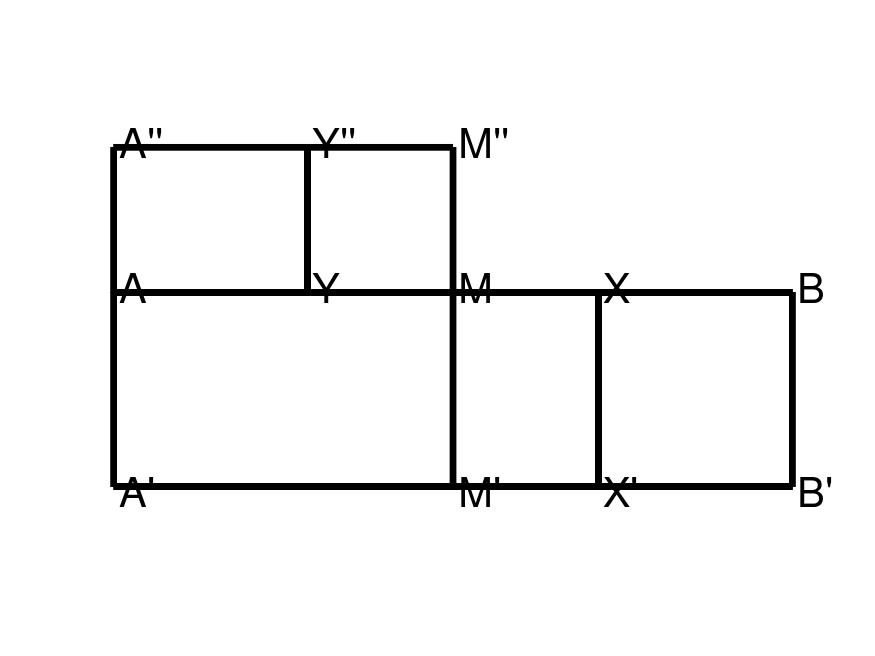
\includegraphics[width=0.48\textwidth]{Storia_della_matematica/Immagine_Fibonacci_SecondoGradobis.png}
	\caption{Risoluzione dell'equazione di secondo grado secondo la quarta forma normale, seconda parte.}
	\label{Fibonacci_SecondoGradobis}
\end{wrapfigure}
\par Costruiamo i quadrati $A'M'M''A''$ e $YMM''Y''$, dove $Y$ \`e il simmetrico di $X$ rispetto ad $M$. Allora il rettangolo $AYY''A''$ \`e congurente al rettangolo $MXX'M'$. Ne deduciamo che $AM^2 = AX \cdot XX' + MX^2$, da cui $\left ( \frac{b}{2} \right )^2 = c + MX^2$, da cui $x = MB - MX = \frac{b}{2} - \sqrt{ \left ( \frac{b}{2} \right )^2 - c}$ e questo conclude la dimostrazione.
\par La dimostrazione per l'altra radice \`e del tutto analoga e riportiamo solamente la figura (figura \ref{Fibonacci_SecondoGradoDue}; il segmento $AA'''$ \`e uguale a $AM$): lo stesso al-Khw\=arizm\={\i} non riporta la dimostrazione, ma le traduzione latine, come noi, riportano la figura. Il ragionamento cambia solo per la seconda parte in maniera immediata: $MX^2 = AM^2 - AX \cdot XX'' - X'''M''' \cdot M'''M'' = AM^2 - AX \cdot XX'' - A''X'' \cdot X''X' = AM^2 - AX \cdot XX' = \left ( \frac{b}{2} \right )^2 - c$.
\begin{wrapfigure}{R}{0.5\textwidth}
	\includegraphics[width=0.48\textwidth]{Storia_della_matematica/Immagine_Fibonacci_SecondoGradoDue.png}
	\caption{Risoluzione dell'equazione di secondo grado secondo la quarta forma normale, seconda radice.}
	\label{Fibonacci_SecondoGradoDue}
\end{wrapfigure}
\par Vediamo la seconda forma normale: in tal caso la soluzione \`e $\sqrt{c + \left ( \frac{b}{2} \right )^2} - \frac{b}{2}$. Abbiamo in questo caso due dimostrazioni geometriche.
\begin{wrapfigure}{R}{0.5\textwidth}
	\includegraphics[width=0.48\textwidth]{Storia_della_matematica/Immagine_Fibonacci_SecondoGrado2.png}
	\caption{Risoluzione dell'equazione di secondo grado secondo la quinta forma normale.}
	\label{Fibonacci_SecondoGrado2}
\end{wrapfigure}
\par La prima \`e illustrata dalla figura \ref{Fibonacci_SecondoGrado2}: si costruisce il quadrato di lato $x$ e sui suoi lati si costruiscono i rettangoli di altezza $\frac{b}{4}$. Allora l'area del quadrato di lati neri \`e $x^2 + 4 \cdot \frac{b}{4}x + 4 \cdot \left ( \frac{b}{4} \right )^2 = x^2 + bx + \left ( \frac{b}{2} \right )^2$. D'altra parte, essendo $x^2 + bx = c$, abbiamo che l'area del quadrato nero \`e $c + \left ( \frac{b}{2} \right )^2$. Se ne deduce che il lato del quadrato nero \`e $\sqrt{c + \left ( \frac{b}{2} \right )^2}$ e dunque il lato del quadrato blu $x = \sqrt{c + \left ( \frac{b}{2} \right )^2} - \frac{b}{2}$.
\par La seconda dimostrazione \`e del tutto analoga, ma invece di costruire quattro rettangoli rossi, ne costruisce solo due, su due lati perpendicolari del quadrato blu: aggiungendo il quadratino dell'angolo corrispondente del quadrato nero si ottiene un nuovo quadrato da cui si pu\`o partire per la nuova dimostrazione.
\begin{wrapfigure}{R}{0.5\textwidth}
	\includegraphics[width=0.48\textwidth]{Storia_della_matematica/Immagine_Fibonacci_SecondoGrado3.png}
	\caption{Risoluzione dell'equazione di secondo grado secondo la sesta forma normale.}
	\label{Fibonacci_SecondoGrado3}
\end{wrapfigure}
\par L'ultima forma canonica si risolve geometricamente con l'ausilio della figura \ref{Fibonacci_SecondoGrado3}: abbiamo $AB = x$, $AE = b$, $M$ punto medio di $FD$. I rettangoli rossi sono congruenti, dunque l'area del quadrato blu \`e uguale a quella del quadrato pi\`u piccolo ($\left ( \frac{b}{2} \right )^2$) pi\`u quella del rettangolo $CDEF$ ($(x - b)x = x^2 - bx = c$). Infine $x = AB = BM + MD = \frac{b}{2} + \sqrt{\left ( \frac{b}{2} \right )^2 + c}$, che \`e la soluzione.
\par Notiamo che negli ultimi due casi viene fornita una sola soluzione: ci\`o \`e coerente col fatto che la matematica allora non considerava mai le soluzioni negative, tradizione che durer\`a almeno sino a Descartes.
\par Il trattato \`e chiaramente rivolto ai mercanti, come si deduce subito dalla prevalente tipologia di problemi affrontati, e infatti gli stessi mercanti, dopo un'iniziale diffidenza verso i nuovi simboli rappresentati dalle cifre araboindiane, si convincono rapidamente della superiorit\`a dei metodi ivi esposti per la gestione dei propri affari, in un periodo storico in cui essi si trovano a gestire e registrare una gran quantit\`a di affari su vasta scala geografica. Non mancano dimostrazioni matematiche, come appunto le dimostrazioni geometriche delle formule fornite per risolvere le equazioni di secondo grado, sul modello di quelle di al-Khw\=arizm\={\i}, ma non esiste ancora, in quel periodo storico rimasto orfano della matematica greca, qualcuno che sia in grado di apprezzarle e ancor meno di migliorarle.
\par L'interesse pratico mercantesco e il disinteresse teorico porta alla fondazione delle scuole d'abaco.
\paragraph{Le scuole d'abaco.} Le scuole d'abaco, prodotto naturale del \textit{Liber abaci} pisano e degli interessi mercantili, si sviluppano naturalmente esclusivamente in Italia: un altro importante centro mercantile \`e quello delle Fiandre, ma la lontananza dal mondo arabo rende impossibile la comparsa di un lavoro simile a quello di Fibonacci e, non essendo ancora stata inventata la stampa, la diffusione dei testi \`e troppo ridotta per favorire uno scambio di conoscenze tra i due pi\`u grandi centri mercantili dell'epoca. Per gli stessi motivi, da notare il fatto che il maggior numero di scuola d'abaco sorge nei comuni maggiormente dediti al commercio e in Toscana: cos\`i una delle citt\`a con le migliori scuole d'abaco \`e inevitabilmente la citt\`a di Firenze, dedita al commercio e in Toscana.
\par Si stima che tra la fine del XIII secolo e la prima met\`a del XVI secolo vi erano circa 70 abacisti, quasi tutti maestri d'abaco, divisi in 20 scuole. Nel 1480, pi\`u del 25\% dei giovani istruiti avevan frequentato la scuola d'abaco; nel tardo Cinquecento, a Venezia, si raggiungeva il 40\%.
\par Le scuole possono essere private, pubbliche o anche finanziate parzialmente dal comune e parzialmente da chi le frequenta. Si entra alla scuola d'abaco circa all'et\`a di dieci anni e vi si resta per due, ma entrambi questi dati variano a seconda delle contingenze. Il programma \`e dato, di massima, dal contenuto del \textit{Liber abaci}, privilegiando i problemi di interesse mercantile, ma vi si potevano aggiungere elementi del \textit{Practica geometriae} o lezioni di grammatica, oltre naturalmente alla particolare esperienza del maestro. Come accennato, la matematica insegnata consiste in algoritmi di risoluzione ed esclude le dimostrazioni.
\par Nelle scuole d'abaco studiano grandi personalit\`a come Piero della Francesca e Leonardo da Vinci (1452-1519), i quali sono, oltre che due geni del rinascimento italiano, due esempi del fatto che tra gli studenti di queste scuole non vi sono solo mercanti, ma anche altre persone che si istruiscono fuori dalle universit\`a, dove dominano in lingua latina il diritto, la medicina, la teologia. Altro abacista di rilievo \`e senz'altro Niccol\`o Fontana (1499-1557), meglio conosciuto come Tartaglia, uno dei maggiori protagonisti del rinascimento matematico.
\par Come abbiamo cercato di spiegare, le scuola d'abaco rifondano il sapere matematico, su basi quasi estranee alla matematica greca antica, ma non solo: lo sviluppano anche. In particolare, per esempio, Piero della Francesca tenta di fondare matematicamente la prospettiva nel \textit{De prospectiva pingendi} (1475): l'influsso abacistico \`e evidente nell'impostazione, lontana dal metodo ipotetico deduttivo classico e strutturata in problemi da risolvere; altro esempio rilevante \`e quello dell'algebra, che si pone per la prima volta come la scienza che studia le equazioni a prescindere da qualsiasi applicazione concreta, anch'essa affrontata da Piero della Francesca che tenta di fornire soluzioni generali che funzionano per\`o solo per quelle equazioni che si presentano nel calcolo degli interessi composti: solo successivamente, grazie a Del Ferro (1465 - 1526), Tartaglia, Cardano (1501 - 1576), Ferrari (1522 - 1565) e anche Bombelli (1526 - 1572), che arriver\`a a tentare di introdurre i numeri complessi senza per\`o riuscirvi, si arriver\`a alle formule generali di risoluzione per le equazioni di terzo e quarto grado, con le limitazioni dell'epoca.

\subsubsection{L'umanesimo e il recupero della matematica greca.}\label{LUmanesimoEIlRecuperoDellaMatematicaGreca}
\paragraph{Principi generali dell'umanesimo relativi alla matematica.} L'umanesimo matematico, che possiamo collocare grosso modo nell'Italia del XVI secolo, trae senz'altro le sue origini dal \textit{Liber Abaci} e dalle scuole d'abaco: \`e attraverso questi due elementi che nasce una nuova generazione di matematici, i quali, come gli artisti e letterati loro contemporanei (quando non sono artisti o letterati essi stessi) si sentono inevitabilmente attratti dal mondo classico. Si pongono dunque, per quanto riguarda l'ambito matematico, i seguenti problemi:
\begin{itemize}
	\item il reperimento di manoscritti greci;
	\item la loro traduzione;
	\item la loro comprensione.
\end{itemize}
\par Nella sottosezione \ref{LaTraditioDellOperaDiArchimedeDiApollonioEDiPappo} vedremo esempi concreti di come sono state affrontate queste problematiche; qui diamo delle linee generali.
\par Com'\`e noto il sapere dei greci non viene perduto con l'ascesa n\'e con la caduta della civilt\`a romana, bens\`i viene conservato dalla civilt\`a araba, che ne promuove lo studio. Gli arabi traducono molti lavori, ma il loro spirito \`e pragmatico, anche quando rivolto alla teoria, non certo umanistico: essi sono interessati esclusivamente a capire i testi, quindi a migliorarli aggiungendovi il proprio contributo, non certo a condurre ricerche filologiche. Questo spirito \`e comunque sufficiente perch\'e i califfi impieghino grandi sforzi per recuperare numerosi manoscritti, per esempio dall'impero bizantino, ne promuovano la traduzione, tipicamente in due fasi, affidandoli prima a traduttori siriaci (che conoscevano il greco), poi a traduttori arabi, e infine li raccolgano per lo studio in grandi biblioteche (famosa quella di Baghdad tra IX e XII secolo, sotto il califfato abbaside).
\par Accanto alle corti di Federico II di Svevia e poi di Carlo di Angi\`o che diedero grande impulso alla diffusione della cultura grecoaraba (abbiamo gi\`a citato i contatti di Fibonacci con Federico II), il principale centro di traduzione dei testi greci ed arabi \`e la penisola iberica: i signori arabi incoraggiano il lavoro scientifico e inevitabilmente il mondo cristiano ne viene attratto; emblematico in questo senso il caso di Gerbert d'Aurillac, il futuro papa Silvestro II, che cerca di diffondere gi\`a prima di Fibonacci il sistema numerico posizionale. Oltre a Gerbert d'Aurillac ricordiamo Adelardo di Bath, il gi\`a citato traduttore di Euclide. E vengono tradotti in latino moltissimi testi greci: gli \textit{Elementi} di Euclide, il \textit{De mensura circuli} di Archimede, l'\textit{Almagesto} di Tolomeo; accanto a questi si aggiungono opere originali arabe come i lavori di al-Kh\=arizm\={\i}.
\par Quindi, come si vede, le opere della matematica greca (e non solo) arrivano in Europa tradotti ben prima dell'umanesimo, ma come dovrebbero far capire il confronto tra Gerbert d'Aurillac e Fibonacci e la \textit{traditio} euclidea gi\`a esaminata, questo non \`e sufficiente affinch\'e la civilt\`a occidentale le capisca e le assimili: le scuole d'abaco costituiscono la premessa necessaria a questo particolare passaggio. Gi\`a nel caso degli \textit{Elementi} di Euclide abbiamo visto che \`e il maestro d'abaco Tartaglia a trovare per primo un equilibrio tra filologia e matematica dando cos\`i un contributo decisivo alla restituzione dell'opera. Nel seguito, descriviamo due personalit\`a protagoniste dell'umanesimo matematico: Commandino e Maurolico.
\paragraph{Federico Commandino (1509 - 1575).} Commandino \`e un umanista che frequenta le corti rinascimentali: viene contatto dal cardinale Cervini della biblioteca Vaticana affinch\'e egli spieghi il senso di due manoscritti compresi in un codice di Moerbeke\footnote{\CFR\ sottosezione \ref{LaTraditioDellOperaDiArchimedeDiApollonioEDiPappo}.} -- i \textit{Galleggianti} di Archimede e \textit{De analemmate}, un'opera astronomica di Tolomeo. Egli riesce a pubblicare la sua edizione dei \textit{Galleggianti} circa quindici anni pi\`u tardi nel 1565: in effetti Commandino si rende rapidamente conto di non avere le conoscenze necessarie per capire e quindi restituire correttamente il testo; egli si dedica dunque ad un lungo lavoro preliminare, prima di ricerca di manoscritti, poi di traduzione e comprensione, che porta alla pubblicazione dei seguenti lavori:
\begin{itemize}
	\item la \textit{Archimedis operis non nulla} (1558), che comprende la traduzione di numerosi lavori di Archimede;
	\item il \textit{Liber de centro gravitati solidorum} (1565), opera originale di Commandino, edita insieme ai \textit{Galleggianti}, volta a spiegare il risultato non dimostrato sul centro di gravit\`a del paraboloide;
	\item un'edizione dei primi quattro libri delle \textit{Coniche} di Apollonio (1566), comprendente una traduzione, un commento, lemmi di Pappo e due testi di Sereno (\textit{De sectione coni} e \textit{De sectione cylindri})\footnote{Non \`e per\`o la prima edizione a stampa: la prima \`e quella stampata a Venezia nel 1537, tradotta dal latino da Giovanni Battista Memmo. Anche Maurolico compie una traduzione dei primi quattro libri a cui aggiunge una ricostruzione dei due successivi: ci\`o avviene nell'anno 1547, ma la pubblicazione \`e del 1654.}.
\end{itemize}
\par Commandino usa la stessa metodologia per l'edizione del \textit{De analemmate} (1562), preceduto del \textit{Planisphaerium} di Tolomeo (1558)\footnote{La prima edizione latina \`e del 1507.}; egli sottolinea inoltre i legami dei problemi affrontati da Tolomeo con quelli della contemporanea prospettiva pittorica.
\par Commadino traduce anche l'opera di Pappo, che viene pubblicata postuma nel 1588 a spese di Francesco II duca di Urbino.
\par L'impostazione di Commandino \`e chiaramente filologica: nel \textit{Liber de centro gravitati solidorum}, di cui egli stesso \`e autore, si nota la volont\`a di rimanere molto vicino al modello archimedeo, modello che contribuisce dunque a imporre nella matematica rinascimentale.
\paragraph{Francesco Maurolico (1494 - 1575).} Maurolico \`e un matematico messinese con un approccio sensibilmente diverso da quello di Commandino o di Tartaglia, pi\`u vicino a quello del mondo arabo altomedievale: egli diffonde s\`i gli scritti dei matematici greci, ma in una forma nuova e riattualizzata. Lavora tutta la vita in Sicilia, effettuando solo pochi viaggi, rimanendo dunque estraneo ai principali centri umanistici, ci\`o che spiega la sua impostazione particolarmente originale.
\par Maurolico adotta un'impostazione enciclopedica: egli studia tutto il sapere matematico (e non solo) a sua disposizione. Emblematico del suo approccio \`e il suo lavoro su Archimede: egli comincia a studiare l'\textit{Equilibrio dei piani} gi\`a prima del 1529, ma solo nel 1544 ne pubblica una prima edizione che diventa il postumo \textit{Archimedis de momentis aequalibus ex traditione Francisci Maurolyci} (1628): si tratta di un'opera in quattro libri molto lontana dal lavoro originale di Archimede. Esso \`e cos\`i strutturato:
\begin{itemize}
	\item libro I: equilibrio, momento, legge della leva;
	\item libro II: centro di gravit\`a dei poligoni;
	\item libro III: centro di gravit\`a della parabola;
	\item libro IV: determinazione del centro di gravit\`a di alcuni solidi (nell'edizione postuma l'autore aggiunge il caso del paraboloide).
\end{itemize}
\par Il \textit{De momentis} mostra chiaramente che Maurolico individua nell'originale i principi teorici fondamentali (simmetrie, momenti) e li rifonde in maniera pi\`u unitaria e in un certo senso moderna.
\par Le opere di Maurolico purtroppo non sono stampate per molto tempo, ma esercitano comunque una certa influenza dopo la morte del loro autore grazie all'amico Cristoforo Clavio (1537 - 1612) che basa su di esse l'insegnamento matematico rivolto alla Compagnia di Ges\`u.

\subsubsection{L'invenzione della stampa e la diffusione della cultura scientifica.}\label{LInvenzioneDellaStampaELaDiffusioneDellaCulturaScientifica}
\paragraph{Primato veneziano.} Intorno all'anno 1450 viene inventata la stampa e in breve tempo Venezia si afferma come una delle pi\`u importanti capitali europee dell'editoria umanistica: tra il 1470 e il 1500 si calcola che a Venezia lavorassero circa 200 tipografie, contro le 60 di Milano, le 30 di Firenze; anche oltr'alpe il confronto \`e impressionante considerando che circa 200 erano le tipografie nell'intera Germania e a 150 ammontavano quelle di Lione e Parigi insieme. Questo \`e dovuto a numerosi fattori:
\begin{itemize}
	\item l'umanesimo ha coinvolto molte citt\`a, tra le quali Firenze, Roma, Urbino e appunto Venezia. A Venezia il cardinale Basilio Bessarione (1403 - 1472), metropolita di Nicea prima del suo trasferimento in Italia nel 1440, ha raccolto un gran quantit\`a di manoscritti greci e li dona alla sua morte a San Marco, accessibile al pubblico dalla met\`a del Cinquecento e di cui si occupa anche Pietro Bembo (1470 - 1547);
	\item la posizione geografica \`e ideale per il reperimento dei manoscritti e per la diffusione delle loro edizioni;
	\item la Repubblica di Venezia incoraggia e promuove la stampa;
	\item il Veneto \`e ricco di cartiere;
	\item il vicino Studio di Padova contribuiva alla domanda di testi, sia per gusto che per l'insegnamento;
	\item un alto livello di istruzione dovuto alla presenza di
	\begin{itemize}
		\item scuole d'abaco;
		\item la Scuola di Rialto, che diventa pubblica intorno alla met\`a del Quattrocento, dedita alla filosofia, alla logica, alla geometria;
		\item la Scuola di San Marco, dedita alla grammatica, alla retorica, alla filologia.
	\end{itemize}
	\item la stampa a caratteri mobili arriva a Venezia nel 1469, ma gi\`a prima si stampavano carte da gioco, immagini religiose e anche libretti scolastici.
\end{itemize}
\paragraph{Regiomontano e Ratdolt.} Johannes M\"uller (1436 - 1476), meglio noto come Regiomontano, \`e il primo dei grandi editori scientifici. Egli fa parte del circolo di Bessarione e si convince rapidamente dell'importanza di stampare gli antichi manoscritti matematici greci e non solo: egli apre una tipografia a Norimberga nel 1472 e stampa un programma che comprende numerosi autori greci, tra cui Euclide e Archimede, medioevali, come Giordano Nemorario, e scritti nuovi e originali. Ma la morte prematura di Regiomontano gli impedisce di concretizzare il progetto: \`e Erhardt Ratdolt (1442 - 1528) a raccoglierne l'eredit\`a, tipografo tedesco che lavora a Venezia dal 1475.
\par Purtroppo per\`o, a differenza di Regiomontano, Ratdolt non ha le conoscenze matematiche necessarie per realizzare lo scopo consapevolmente ed egli produce dunque testi come i gi\`a commentati \textit{Elementi} di Euclide (\Cfr\ sottosezione \ref{EuclideEGliElementi}). Le sue tecniche tipografiche sono per\`o eccellenti, soprattutto per le sue stampe iconografiche: egli stampa immagini astronomiche, immagini policrome, impiega l'oro.
\par Dopo Ratdolt, altri editori intraprendono progetti di edizioni enciclopediche:
\begin{itemize}
	\item Giorgio Valla (1447 - 1500) pubblica \textit{De expedentis et fugiendi rebus opus}, ricco di molte nuove traduzioni dal greco in latino anche di testi matematici;
	\item Paganino de' Paganini pubblica la \textit{Summa de arithmetica, geometria, proportioni et proportionalita} di Luca Pacioli (1445 - 1517), in lingua volgare, con cui l'autore mira a superare la matematica pragmatica delle scuole d'abaco reintegrandola col sapere teorico. La \textit{Summa} include molti passi dell'edizione campana degli \textit{Elementi} di Euclide; oggi Pacioli viene ``accusato'' di aver plagiato i risultati dei maestri d'abaco, tra i quali quelli del suo maestro Piero della Francesca, bench\'e si debba tenere a mente che \`e proprio con l'invenzione della stampa che nascono i primi concetti legati al diritto d'autore\footnote{A Tartaglia per esempio vengono riconosciuti a Venezia diritti esclusivi di stampa della propria opera.}.
\end{itemize}


\subsection{Dalla riappropriazione dei classici a nuovi orizzonti metodologici.}\label{DallaRiappropriazioneDeiClassiciANuoviOrizzontiMetodologici}
\subsubsection{La \textit{traditio} dell'opera di Archimede, di Apollonio e di Pappo.}\label{LaTraditioDellOperaDiArchimedeDiApollonioEDiPappo}
\paragraph{Il codice Moerbeke.} La \textit{traditio}, cio\`e la tradizione, delle opere degli antichi matematici greci ruota attorno a quella di coloro che furono forse i pi\`u grandi matematici dell'antico mondo greco: quella degli \textit{Elementi} di Euclide, che abbiamo gi\`a esaminato ampiamente nella sottosezione \ref{EuclideEGliElementi}, e quella dei lavori di Archimede, a cui abbiamo gi\`a dato alcuni accenni e che esaminiamo pi\`u approfonditamente adesso.
\par Nel corso del basso medioevo, come si \`e visto, la scena matematica \`e dominata dalla scuole d'abaco e dunque da un approccio pragmatico e dunque pragmatico \`e anche l'interesse manifestato nei confronti dei pochi scritti di Archimede che circolano, dai quali gli abacisti traggono, essenzialmente, le formule per il calcolo della circonferenza, del cerchio, della sfera e della palla, senza curarsi troppo di comprenderne la provenienza.
\par Uno dei pochi personaggi che si dedica ad uno studio completo dell'opera di Archimede \`e il domenicano Guglielmo di Moerbeke (circa 1215 - 1286). Egli, lavorando presso la corte papale di Viterbo, prepara un codice che contiene la traduzione di due manoscritti greci, oggi perduti, contenenti alcuni testi di Archimede e alcuni commenti. L'opera \`e particolarmente importante perch\'e lo stile di Gugliemo \`e molto vicino a quello degli originali, cosa che compensa la perdita degli originali stessi e perch\'e i \textit{Galleggianti} ci erano pervenuti solo tramite uno dei due manoscritti greci in questione e sarebbero dunque andati perduti senza il codice Moerbeke. Grazie a Guglielmo, alla fine del 1269 tutta l'opera di Archimede oggi pervenutaci, all'eccezione dell'\textit{Arenario} e del \textit{Metodo}, \`e disponibile ai matematici tardomedievali, che per\`o abbiamo visto essere maestri d'abaco tesi all'utilit\`a pratica e dunque ancora impreparati ad accogliere l'impostazione teorica degli antichi. Inoltre, l'ambiente propizio allo sviluppo matematico della corte di Viterbo si interrompe presto a causa della cattivit\`a avignonese (1309 - 1377). Il contesto europeo \`e ulteriormente turbato dalla Guerra dei Cent'anni (1337 - 1453), nonch\'e dalla peste nera (1348). Tutto ci\`o ha per risultato che il codice di Moerbeke rimane pressoch\'e ignorato sino al XIV secolo, eccezion fatto per una copia della traduzione delle \textit{Spirali}, chiaramente di scarso interesse per l'epoca.
\paragraph{Da Iacopo di San Cassiano (circa 1415 - circa 1452) a Tartaglia.} Il papa Niccol\`o V (1397 - 1455) \`e un grande sostenitore dell'umanesimo ed \`e infatti il fondatore della Biblioteca Vaticana. \`E proprio per la Biblioteca Vaticana che Niccol\`o V commissiona a Iacopo di San Cassiano una traduzione dell'opera di Archimede: la traduzione che ne risulta viene rivista e corretta attorno al 1462 da Regiomontano, venuto in Italia insieme al gi\`a citato cardinale Bessarione; Regiomontano si serve, tra altri documenti, di uno dei manoscritti che aveva utilizzato anche Gugliemo da Moerbeke, e forse della traduzione di Guglielmo stesso. Regiomontano vorrebbe sfruttare la stampa per pubblicare un'edizione delle opere di Archimede, ma purtroppo muore nel 1476; il suo lavoro viene comunque utilizzato per l'\textit{editio princeps} grecolatina di Basilea (1543 - 1544).
\par A partire dalla traduzione di Iacopo da Cassiano, gli abacisti, sia pure sempre orientati ad interessi pratici, cominciano ad interessarsi maggiormente ai lavori di Archimede. In particolare,
\begin{itemize}
	\item Piero della Francesca dimostra di aver studiato Archimede nel suo \textit{Libellus de quinque corporibus regularibus} e si discute anche di un codice della biblioteca riccardiana di Firenze di cui egli potrebbe essere l'autore e che attesterebbe anch'esso gli interessi archimedei di Piero;
	\item Leonardo da Vinci propone una dimostrazione riguardo alla posizione del centro di gravit\`a del triangolo nel \textit{Codice Arundel}, anche se ingenua rispetto allo stile di Archimede.
\end{itemize}
\par Gli abacisti non sono dunque ancora in grado di apprezzare a pieno gli scritti di Archimede, ma l'interesse \`e ormai nato. Notevole il codice M, citato anche da Leonardo, usato da Luca Gaurico (1475 - 1558) per la pubblicazione del \textit{Tetragonismus} (Venezia, 1503), contenente la \textit{Quadratura della parabola} e la \textit{Misura del cerchio}: sebbene il \textit{Tetragonismus} sommi gli errori del codice M, di Gaurico e dello stampatore, esso resta comunque la prima stampa di testi archimedei.
\par Ma i lavori di Archimede si diffondono ancora di pi\`u con l'opera di Tartaglia, che dedica molto impegno ai testi del grande matematico di Siracusa:
\begin{itemize}
	\item reperimento nel 1531 di una copia latina del primo libro de \textit{La sfera e il cilindro};
	\item pubblicazione dei lavori di Archimede nel 1543 - 1544, basata sul codice M -- unica edizione sino al 1565 ad includere i \textit{Galleggianti};
	\item pubblicazione di un'edizione in volgare dei \textit{Galleggianti} nel 1551 in \textit{Ragionamenti intorno alla sua travagliata inventione};
	\item pubblicazione postuma (1557) di una parafrasi in volgare de \textit{La sfera e il cilindro} in \textit{General trattato di numeri e misure}.
\end{itemize}
\par Abbiamo gi\`a visto che la trasmissione dei testi archimedei porta alla trasmissione anche di quelli apolloniani e pappiani. Per ulteriori dettagli sulla \textit{traditio} di questi autori, rimandiamo alla sottosezione \ref{LUmanesimoEIlRecuperoDellaMatematicaGreca}.

\subsubsection{Il problema dei centri di gravit\`a e l'opera di Luca Valerio.}\label{IlProblemaDeiCentriDiGravitaELOperaDiLucaValerio}
\par La \textit{traditio} archimedea ha portato con s\'e, fra gli altri, il tema della ricerca dei centri di gravit\`a: questo \`e uno dei primi temi affrontati dai matematici del Cinquecento.
\par Una delle figure pi\`u importanti in questo ambito \`e Luca Valerio (1553 - 1618), allievo di Clavio e dunque, indirettamente, di Maurolico. Egli affronta nel suo \textit{De centro gravitatis solidorum libri tres} il problema della ricerca dei centri di gravit\`a di tutti i solidi tradizionali (cubo, piramide, sfera, paraboloide...) e delle loro parti, che era stato risolto solo parzialmente da Archimede; Valerio per\`o guarda al problema in maniera completamente nuova: egli inventa un metodo generale.
\par Valerio parte dai lavori di Archimede e da quelli di Commandino e coglie la generalit\`a dei loro metodi: egli pertanto, per la prima volta nella Storia della matematica compie il passo di introdurre oggetti generali, definiti da una propriet\`a, che consenta di enunciare teoremi generali dai quali conseguono automaticamente i teoremi di Archimede e Commandino riguardo alle figure particolari da essi studiate. Valerio considera una classe di figure piane e una classe di solidi che definisce digradanti rispettivamente
\begin{itemize}
	\item \textit{circa diametrum}: sono le figure piane che presentano un diametro, cio\`e una retta che biseca qualsiasi corda della figura;
	\item \textit{circa axim}: si tratta dei solidi che presentano un asse di simmetria (la retta che congiunge i centri di due basi opposte o un vertice e il centro della base corrispondente) e che, quando vengono tagliati da un piano che scorre lungo quest'asse, presentano sezioni simili ma di area sempre minore.
\end{itemize}
\par Il passo successivo consiste nell'enunciare e dimostrare teoremi sulle figure digradanti: per esempio, un teorema afferma che due figure avente stesso asse e sezioni proporzionali hanno lo stesso centro di gravit\`a.
\par Chiaramente, queste sezioni anticipano il principio degli indivisibili di Cavalieri, tuttavia Valerio rimane ancorato alla tradizione e cerca nella geometria classica la giustificazione dei suoi metodi e inoltre rimane comunque legato all'antico problema dei centri di gravit\`a, non va oltre ad esso.
\par Valerio \`e anche considerato da alcuni il vero inventore del metodo di esaustione (non \`e forse un caso se ad inventare questo termine sar\`a Gr\'egoire de Saint-Vincent, anch'egli della scuola di Clavio). Come sappiamo, il metodo di esaustione \`e gi\`a stato usato spesso dagli antichi, e in particolare da Archimede, ma si tratta pi\`u di uno stile dimostrativo, da riadattare caso per caso, che un metodo generale. Questo invece \`e il metodo di esaustione di Valerio: per conoscere il rapporto tra due grandezze $A$ e $B$, basta approssimarle con due grandezze $E$ ed $F$ -- cio\`e scegliere due grandezze $E$ ed $F$ tali che $A - E$ e $B - F$ possano essere resi piccoli a piacere -- e si avr\`a che il rapporto cercato \`e lo stesso che intercorre tra $E$ ed $F$.
\par Accenniamo infine che, nonostante il problema dei centri di gravit\`a sia legato alla forma dei solidi coinvolti, Valerio inizia a staccarsi dal concetto di forma per concentrarsi sul concetto di quantit\`a, prendendosi libert\`a di comporre e scomporre le figure secondo necessit\`a, sebbene egli ritenga che questo metodo, essendo lontano dallo stile archimedeo che costituisce il suo riferimento, non sia legittimo, un po' come il \textit{Metodo meccanico} di Archimede (che Valerio non conosceva) era considerato solo un mezzo matematico euristico dal suo stesso autore.
\par Per il suo stile, vicino a quello degli antichi e in particolare di Archimede, Valerio pu\`o essere considerato l'ultimo geometra della misura, ma per i suoi contenuti innovativi egli \`e anche il primo dei moderni analisti: dai suoi lavori infatti prender\`a le mosse Bonaventura Cavalieri.

\subsubsection{Fran\c{c}ois Vi\`ete e l'invenzione dell'algebra simbolica.}\label{FrancoisVieteELInvenzioneDellAlgebraSimbolica}
\paragraph{Prima di Vi\`ete.} Come abbiamo visto, la matematica greca \`e molto pi\`u interessata alla geometria che all'aritmetica ed \`e dunque naturale che essa non abbia sviluppato quasi nessun simbolismo, se si escludono gli enti geometrici rappresentati da lettere proprio come oggi. Bisogna comunque notare l'eccezione di Diofanto (III - IV secolo a.c.) che nel suo \textit{Arithmetica} fa uso sistematico di simboli per rappresentare numeri ed operazioni: sebbene i simboli da lui scelti non siano i pi\`u efficienti (manca per esempio la notazione posizionale), essi si rivelano comunque efficaci. \`E infatti proprio da Diofanto che partir\`a Vi\`ete per la sua proposta.
\par La matematica medievale dimostra interessi diversi rispetto a quelli greci, e cos\`i, come abbiamo visto, a seguito della pubblicazione del \textit{Liber abaci} si impone rapidamente l'uso del sistema numerico decimale posizionale. Inoltre, sempre grazie agli arabi, inizia a svilupparsi tra gli abacisti una corrente algebrica, che richiede un linguaggio meno retorico e pi\`u efficiente: non si arriva ancora ad un linguaggio simbolico, ma si iniziano ad abbrevviare le operazioni pi\`u comuni ($p$ per ``pi\`u'', $m$ per ``meno''), si introducono parole chiave come \textit{res} e \textit{census}\footnote{Il loro uso definisce la \Define{notazione cossica}, dalla traduzione della parola latina \Define{res} in lingua tedesca.} -- per indicare rispettivamente l'incognita e il suo quadrato --, simboli per abbreviarle e si cominciano anche a denotare con esponenti le potenze dell'incognita. \`E in questo contesto che si muove Fran\c{c}ois Vi\`ete.
\paragraph{Fran\c{c}ois Vi\`ete (1540 - 1603)} Vi\`ete desidera restituire il sapere degli antichi riattualizzandolo e cerca di ritrovare quei risultati a cui Diofanto fa spesso riferimento senza per\`o dimostrarli: \`e questo lo spirito con cui scrive \textit{In artem analyticam isagoge} (1591). \`E cos\`i che nasce la sua idea pi\`u innovativa: utilizzare simboli non solo per incognite e operazioni, ma anche per i coefficienti stessi delle equazioni. Vi\`ete sceglie di indicare con consonanti le quantit\`a note (con segno positivo: egli non introduce mai parametri negativi) e con vocali quelle ignote\footnote{A Descartes \`e dovuto l'uso attuale di indicare le quantit\`a note con le prime lettere dell'alfabeto e le incognite con le ultime.} e distingue tra
\begin{itemize}
	\item \textit{logistica numerosa}, che studia equazioni i cui coefficienti sono tutti numeri ben fissati, come \`e sempre stato fatto sino ad allora;
	\item \textit{logistica speciosa}, che studia equazioni i cui coefficienti sono simboli.
\end{itemize}
\par Vi\`ete non considera i parametri come numeri fissati qualunque, ma come veri e propri parametri: egli \`e perfettamente consapevole che non sta pi\`u studiando equazioni particolari, ma vere e proprie classi di equazioni. \`E il passaggio dall'aritmetica e da una forma primitiva di algebra, all'algebra simbolica.
\par Grazie a questo nuovo linguaggio, Vi\`ete riesce a dimostrare in piena generalit\`a identit\`a come quelle date dai prodotti notevoli.

\subsubsection{La meccanica: da Giordano a Galileo.}\label{LaMeccanicaDaGiordanoAGalileo}
\paragraph{Giordano Nemorario (XIII secolo).} Gli antichi, sia pure con notevoli eccezioni come quella di Archimede, si sono dedicati poco allo studio della meccanica: Aristotele ha illustrato una meccanica che spiega le cause del moto e nulla di pi\`u viene ricercato: gli oggetti hanno delle qualit\`a, come la pesantezza, e vanno laddove le loro qualit\`a li spingono; l'aria e il fuoco sono dotati di leggerezza e vanno verso l'alto, l'acqua e la terra di pesantezza e vanno verso il basso. Le teorie fisiche rimangono pressoch\'e immutate sino al XIII secolo. Giordano Nemorario \`e uno dei primi a cambiare le cose.
\par Poco si sa della vita di Giordano Nemorario, ma i suoi scritti sono senza dubbio molto influenti: essi sono citati da Ruggero Bacone (1214 - 1294) e sono fra i primi testi dati alle stampe nel Cinquecento. Giordano, studiando le leve, inventa il concetto di \textit{gravitas secundum situm}, che possiamo confrontare con la \textit{gravitas secundum speciem} esposta nel \textit{Liber archimenedis de ponderibus}, di autore ignoto:
\begin{itemize}
	\item secondo la \textit{gravitas secundum situm} un corpo \`e tanto pi\`u pesante quanto pi\`u la sua ``linea di moto'' \`e prossima alla verticale; per esempio \`e molto faticoso sollevare un masso lungo la verticale, ma lo \`e molto meno spingerlo orizzontalmente o lungo un piano inclinato; tanto pi\`u \`e inclinato il piano, cio\`e la sua linea di moto \`e vicina alla verticale, tanto pi\`u il corpo \`e pesante. Sulla base di questo principio, che Giordano adopera come un assioma, egli riesce a dimostrare alcuni risulati sui piani inclinati;
	\item la \textit{gravitas secundum speciem} invece anticipa il concetto di peso specifico: questo concetto stabilisce che per confrontare il peso di due materie si devono paragonarne quantit\`a uguali in volume. Manca la definizione esplicita di peso specifico come rapporto, ma l'idea \`e introdotta.
\end{itemize}
\paragraph{Il Cinquecento.} Nel Cinquecento ricompare un trattato pseudoaristotelico intitolato \textit{Quaestiones Mechanicae}: la prima pubblicazione, in greco, avviene a Venezia nel 1497; seguono una traduzione in latino a Parigi di Vittore Fausto nel 1517 e vari commenti e parafrasi. Notevoli sono la parafrasi di Alesandro Piccolomini (Roma, 1547) -- che attribuisce in introduzione alla meccanica, sino ad allora considerata un'arte manuale, la dignit\`a di scienza che consente all'Uomo di superare con le sue forze le forze della Natura -- e la parafrasi di Tartaglia in \textit{Quesiti et inventioni diverse} (Venezia, 1546 e 1554), che riprende anche le teorie di Giordano sui pesi.
\par Tutto ci\`o che abbiamo descritto sin'ora, da Giordano Nemorario ai \textit{Quesiti et inventioni diverse}, ha poco in comune con la filosofia naturale degli antichi: il primo a tentare una sintesi tra l'impostazione aristotelica e quella archimedea (e neoarchimedea) \`e Guidobaldo dal Monte (1545 - 1607), allievo di Commandino, amico e mentore di Galileo. Guidobaldo tenta, in chiave moderna, di ricondurre le macchine alla geometria nel suo \textit{Mechanicorum liber} (Pesaro, 1547; e poi, in volgare, Venezia, 1581), riconducendole tutte alla leva. Tuttavia, egli si dimostra troppo aderente ai classici, tanto da riportare il risultato sbagliato di Pappo sul piano inclinato anzich\'e quello corretto di Giordano.
\par Pi\`u tardi, nel 1588, Guidobaldo pubblica a Pesaro, proseguendo l'opera archimedea di Commandino, il \textit{Paraphrasis in duos Archimedis aequiponderatium libros}, col quale egli stabilisce la concordanza di Aristotele e Archimede: essi affermano, secondo lui, le stesse cose; laddove il filosofo descrive la macchina attraverso le cause, il matematico la descrive ponendo gli assiomi, in un quadro di ``\textit{maximus consensus}''. Cos\`i Guidobaldo riporta la meccanica nell'ambito della geometria tradizionale, non senza scontrarsi tuttavia col problema delle grandezze derivate che i nuovi lavori hanno cominciato a proporre, come la \textit{gravitas secundum situm} e quella \textit{secundum speciem}: il passo successivo sar\`a compiuto da Galileo.
\paragraph{Galileo Galilei (1564 - 1642).} In un primo momento, col suo \textit{De motu antiquiora}, Galileo rompe con la tradizione aristotelica: egli \`e intento e studiare il moto dei gravi e dei leggeri e considera la possibilit\`a di abbandonare l'idea aristotelica dei leggeri, lasciando solo i gravi, da trattare archimedicamente. \`E una delle prime volte che il matematico non solo descrive il moto, ma ne considera anche le cause; per\`o nei tentativi precedenti si sono presi come punti di partenza i teoremi archimedei: Galileo invece tenta di dimostrare anche quelli.
\par La sua idea \`e quella di partire dai \textit{Galleggianti}: per il giovane Galileo, i corpi leggeri salgono perch\'e scacciati da quelli pi\`u pesanti che premono su di loro. Egli tenta di dimostrare la legge del galleggiamento riconducendola a quella della leva (e dunque l'Archimede dei \textit{Galleggianti} \`e s\'i messo in discussione, ma per essere recuperato attraverso l'Archimede dell'\textit{Equilibrio dei piani}), ma si accorger\`a pi\`u tardi egli stesso di essersi sbagliato. I suoi studi gli permettono comunque di ristabilire la legge corretta per il piano inclinato e costituiscono il primo passo per un modello matematico della Natura completo.
\par La carriera di Galileo prosegue con le lezioni di meccanica a Padova, dove egli insegna con un tale successo che gli appunti sui suoi corsi vengono ampiamente diffusi, bench\'e egli non li publicasse. Nel suo \textit{Mecaniche}, di impostazione simile al guidobaldiano \textit{Mechanicorum liber}, egli rompe definitivamente con la filosofia della Natura: egli si rivolge ad architetti ed ingegneri, non pi\`u a filosofi, e nega che gli effetti delle macchine siano inganni nei confronti della natura. Galileo inoltre introduce per la prima volta, accanto al concetto di gravit\`a, quello di momento, definito come propensione di un corpo ad andare verso il basso: il linguaggio non \`e ancora quello moderno del prodotto vettoriale di oggi, ma egli ha comunque piena consapevolezza del concetto, superando la \textit{gravitas secundum situm} di Giordano.
\par Galileo scriver\`a successivamente i famosi lavori che hanno segnato la Storia della Scienza nello stesso spirito. Va sottolineato per\`o che egli non supera mai l'impostazione archimedea: il suo linguaggio, anche mentre introduce grandezze derivate nuove come appunto il momento, o anche la velocit\`a, l'accelerazione, la forza, resta sempre quello delle proporzioni. Come Valerio, anche Galileo si ferma laddove serve un linguaggio nuovo: il calcolo infinitesimale.


